\section{Scenarios}


The obstruction-free fish-eye lens can be used with different types of volumetric datasets. First, we present a scenario based on baggage inspection (an heterogeneous dataset). Second, we apply our lens technique to a volume of streamlines where the transparency doesn't allow seeing a dense spherical item within its context. Finally, we observe  a special aircraft trajectory within its context inside a dataset representing one day of traffic.

\subsection{Baggage inspection: an unusual blunt object}

\begin{figure*} 
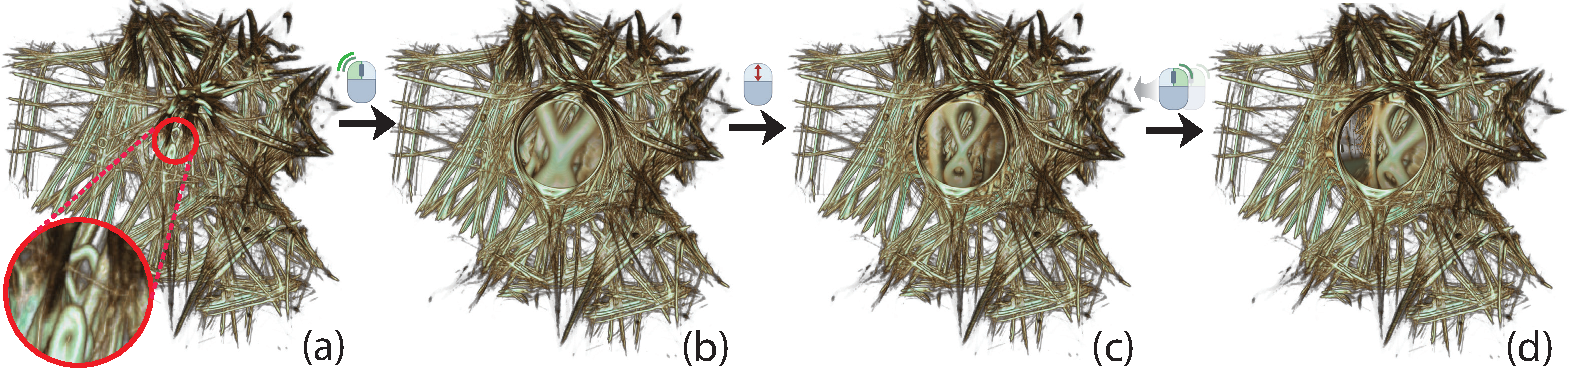
\includegraphics [width=\textwidth]{images/aircraft_lens.pdf} 
\caption{Inspecting an abnormal aircraft trajectory. (a) The initial view on the trajectories where the abnormal trajectory was spotted. (b) The transition  towards a magnified trajectory starts just after the lens tool has been used (double click). (c) The trajectories is magnified. (d) Local Rotations allow to look around the target (right click+ mouse drag toward the desired direction).}
\label{f:aircraft_lens}
\end{figure*}
In most airports, security agents deal with volumetric data exploration during baggage inspections. While automatic systems are now able to detect harmful densities (such as  C-4, TNT, Nitroglycerin, etc.) and event some prohibited articles (such as classical firearms and knives), it remains difficult to identify unusual threats. In addition, baggage inspection faces 4 main concealment strategies:

\textbf{Superposition}: A threat (e.g. prohibited object like a knife, a cutter…) may be sheltered behind dense materials. Sometimes, it’s possible to see through these blind shield using some functionalities such as high penetration (enhanced X-ray power) or image processing (contrast improvement). 

\textbf{Location}: Depending on its location inside the luggage, a threat can be difficult to detect. Objects located in the corners, in the edges or inside the luggage’s frame are very difficult to identify.

\textbf{Dissociation}: Another way to dissimulate a threat is to separate and to spread parts of it in the luggage (weapon or explosive are composed of many separated items like the trigger, the cannon...). This dissociation can be combined with other dissimulation techniques.

\textbf{Lure}: An ill-intentioned individual may use a lure to hide the real threat. For instance, a minor threat like a small scissors may be clearly visible and catch security agent’s attention while a more important threat remains hidden.

As an example, a baggage containing different types of objects as in \autoref{f:baggage_orientation} ( with a volume size of 283x189x344 ) can be declared non-suspect by automatic inspection systems. However, while exploring this baggage with different angles and perspectives, it appears that an object is hidden between a set of mugs. A common solution to this type of issue in baggage inspection is to filter the materials by density in order to show or hide subsets of the volume and reduce the occlusion. But in this case, trying to discriminate the materials on the basis of their densities is not enough to fully reveal the hidden object (\autoref{f:baggage_lens}b-d). In fact, this suspect item shares almost the same density as the surrounding ceramic mugs. 

Using the obstruction-free fish-eye lens can help in this kind of situation. The user has just to use this tool on the partially hidden target. Then, a transition inside the lens will start and smoothly provide the finale unobstructed view of the blunt object which is, in this case, a ceramic shuriken (\autoref{f:baggage_lens}e-g). 



\subsection{Streamlines visualization}



Streamlines visualization has a long history in the scientific visualization community \cite{brambilla2012illustrative}. One of the major challenges is to produce an efficient visualization to display flow directions and their structure in a dense and tangled set of streamlines. In this scenario, we do not claim to propose a new visualization technique, but we rather show how our interactive fish-eye lens can leverage user ability to inspect interesting phenomena within its context (a dense and cluttered streamline dataset). 
\autoref{f:streamLineSTDViz} shows 2 visualizations of our streamline dataset. We use the dataset extracted from  ~\cite{griebel2004flow} which corresponds to a water flow in a basin computed on a  grid of 128x85x42 cells, a set of 4595 stream lines with 183k sampled points. We use an accumulative blending process to distinguish dense areas where many streamlines are aggregated and generate a volume with a size of 500x500x500 voxels. In the first picture \autoref{f:streamLineSTDViz}-a the streamlines are displayed with transparency, which allows noticing a dense spherical item inside the dataset. But when we increase the opacity of the surrounding whirlpool in order to better see its shape and behavior, the spherical item become occluded.
% This visualization suffers from a lack of insight retrieval but it provides evidence of a whirlpool located on the top left part of the image.
Thanks to our interactive lens, the user can distort the view and push on the border of the lens the occluding stream ,and then, inspect this spherical object as well as its context in more details by defining different points of view (\autoref{f:stream_lens}).  Interesting enough, this object corresponds to a streamline with a tiny velocity which makes this line very short. Since every stream in our dataset contains the same number of sampled points, this object has a high density (we used a data convolution technique to turn our vectorial streamline dataset into a volumetric one). In conclusion, our technique eases the detection and the investigation of dataset subset. Other techniques can be applied, but our method is fast and flexible enough to leverage user ability with this streamline dataset exploration.

% \begin{figure} 
% \includegraphics [width=0.45\textwidth]{images/streamLineSTDViz.png} 
% \caption{ This figure shows a standard streamline dataset visualization with a cumulative alpha blending. In the top left part of this image, one can barely distinguish a whirlpool.}
% \label{f:streamLineSTDViz}
% \end{figure} 



\subsection{Unusual aircraft trajectories in French sky}


One of the major issue when visualizing large dataset of moving object is to address the occlusion issue where too many lines spoil their investigation. Many investigations have already been done, especially regarding aircraft movement exploration \cite{hurter2014interactive}.
\begin{figure} 
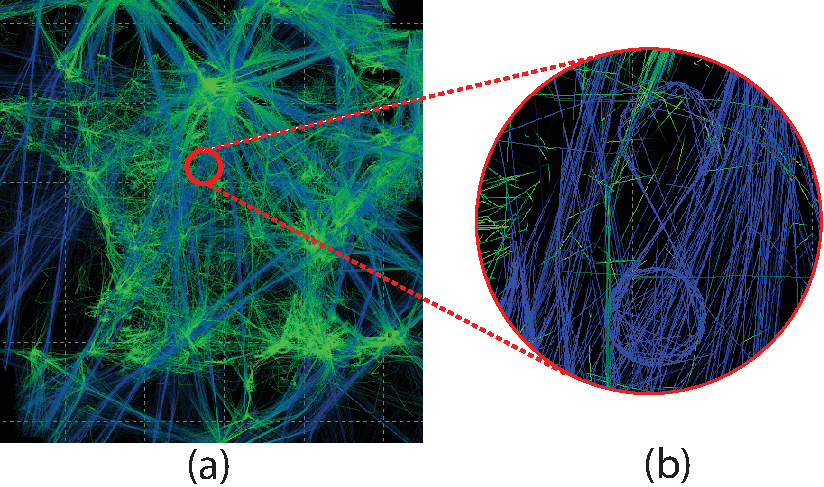
\includegraphics [width=0.45\textwidth]{images/aircraft.pdf} 
\caption{ Standard visualization of one day of recorded aircraft trajectories over France.\cite{hurter2009fromdady}. (a) An unusual trajectory is spotted but needs some manipulation to be unobstructed. (b) Zoom and color filtering technique to visualize abnormal trajectory of one aircraft performing a loop with an eight shape trajectory. This aircraft corresponds to a tanker waiting for refueling other aircraft.}
\label{f:fromdady}
\end{figure}
Figure \autoref{f:fromdady}-a shows one day of recorded aircraft trajectories and \autoref{f:fromdady}(b) shows a subset of such dataset where one can visualize an abnormal aircraft trajectory. A tanker aircraft performed an eight shape loop while waiting to refuel other aircraft. Even if the visualization of such specific trajectory is possible with existing tools, it remains a difficult task which requires time and complex settings. With our technique (with a volume size of 500x500x500), the user can easily spot the corresponding aircraft and even if this trajectory remains barely visible, our lens tools will remove the occluding trajectory thus providing a suitable point of view to fully investigate this trajectory. Furthermore, this obstruction free lens allows to look around the targeted trajectory in order to look for neighboring trajectories.

\begin{figure} 
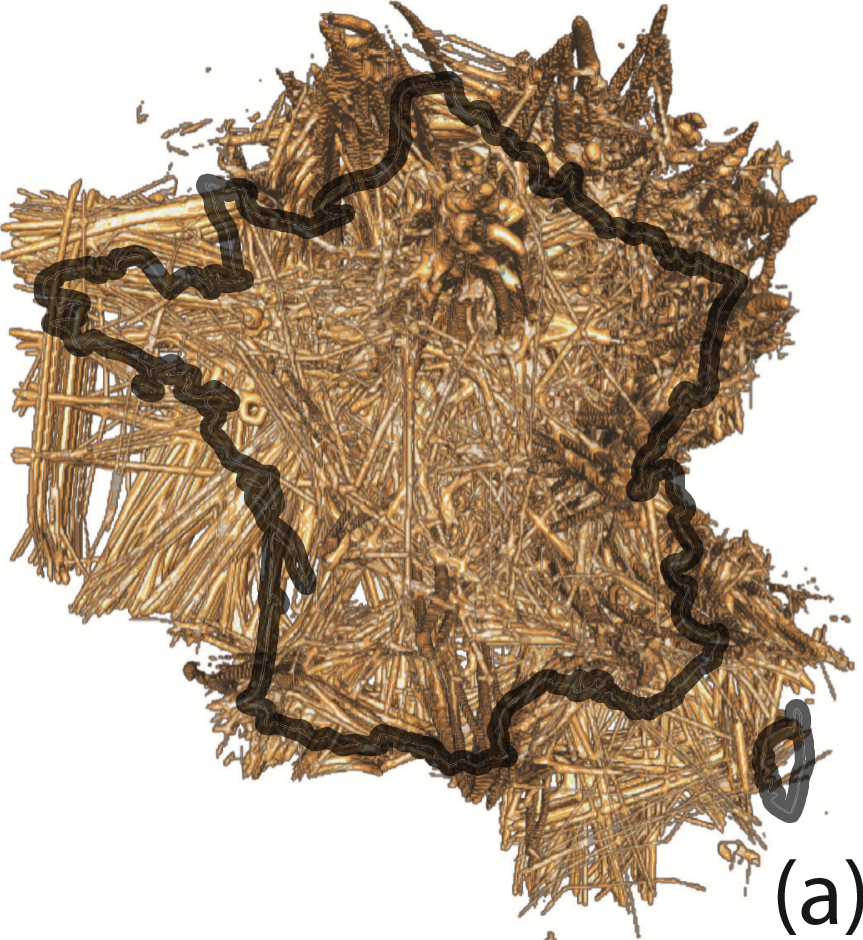
\includegraphics [width=0.36\textwidth]{images/topViewFR.png} 
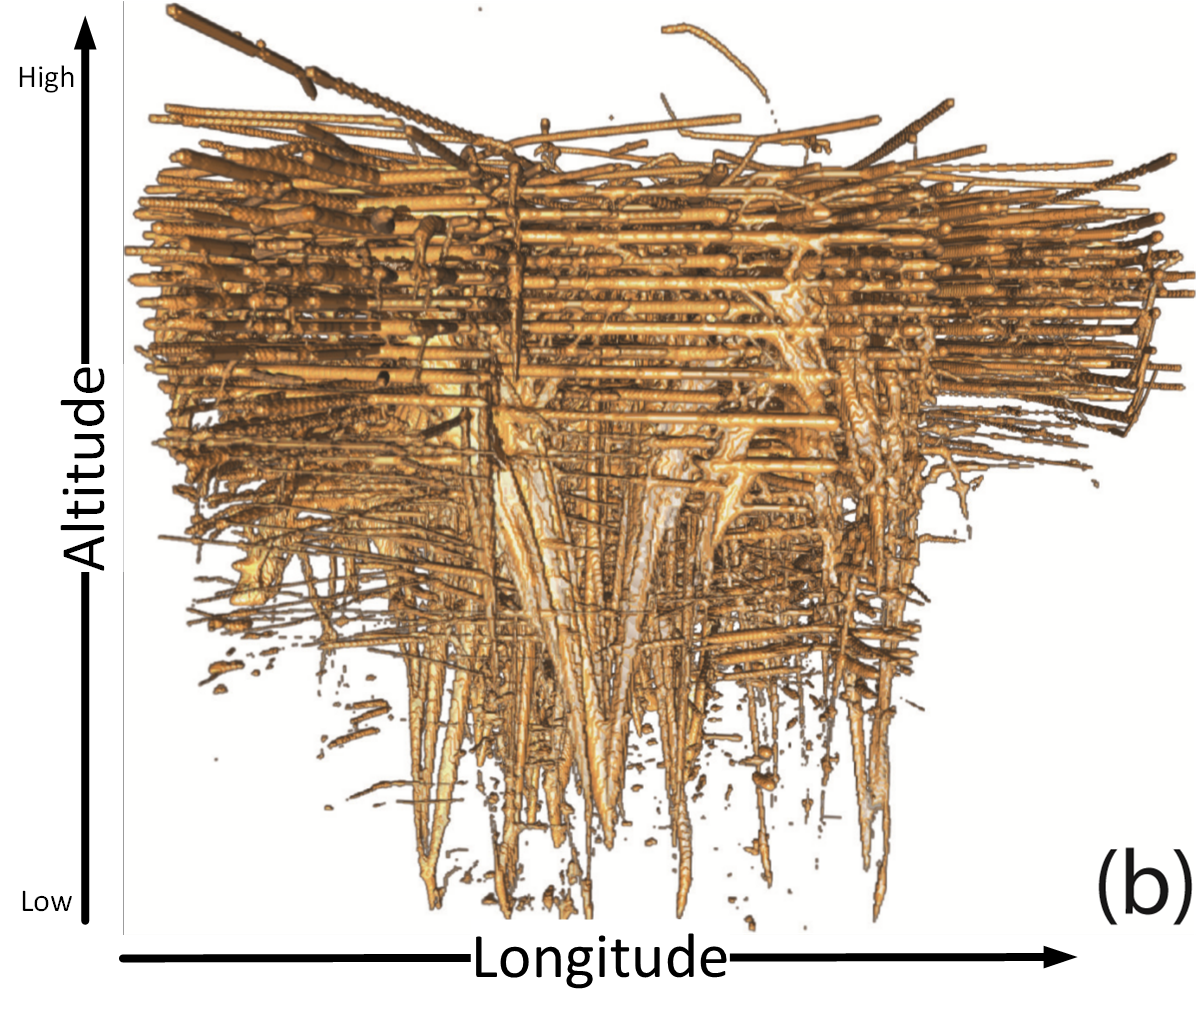
\includegraphics [width=0.4\textwidth]{images/VerticalViewLabel.png} 
\caption{Visualization of one day of recorded aircraft trajectories over France using our volume rendering framework. (a) The trajectories almost draw the map of France. (b) The trajectories are displayed according to their altitudes. }
\label{f:aircraft_orientation}
\end{figure}


